\documentclass{article}

\usepackage[utf8]{inputenc}
\usepackage[turkish, shorthands = :!]{babel}
\usepackage[T1]{fontenc}
\usepackage{lmodern}

\usepackage{fancyhdr, mathtools, tikz, nicefrac}

\usetikzlibrary{arrows.meta} % yönlü okların kafalarının büyüklüğünü ayarlayabilmek için (bk. https://tex.stackexchange.com/a/161238/178454)
\usetikzlibrary{positioning} % düşey ve yatay düğüm mesafelerini farklı belirleyebilmek için (bk. Tikz & PGF kılavuzu, §17.5.3)

\renewcommand{\headrulewidth}{0 pt}
\pagestyle{fancy}
\fancyhf{}
\fancyhead[C]{\thepage}

\begin{document}

%%%%%%% SAYFA 1 %%%%%%%

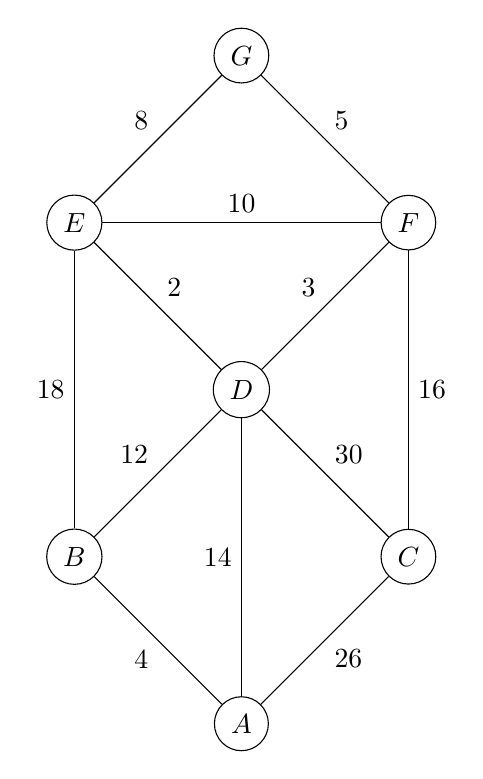
\begin{tikzpicture}[
	node distance = {3 cm},
	vertex/.style = {draw, circle}
	% burada "vertex/.style = {draw, circle}" demeyip aşağıda her "vertex" gördüğümüz yere "draw, circle" yazsak da oluyor
	]
% düğümler
\node [vertex] (A) {$A$}; % \node [<options>] (<name>) at (<coordinate>) {<text>}; (düğüm ismi, seçeneklerden önce de gelebilir)
\node [vertex] (B) [above left of = A] {$B$};
\node [vertex] (C) [above right of = A] {$C$};
\node [vertex] (D) [above right of = B] {$D$};
\node [vertex] (E) [above left of = D] {$E$};
\node [vertex] (F) [above right of = D] {$F$};
\node [vertex] (G) [above right of = E] {$G$};
% arklar
\draw (A) -- node[midway, below left] {4} (B);
\draw (A) -- node[midway, below right] {26} (C);
\draw (A) -- node[midway, left] {14} (D);
\draw (B) -- node[midway, above left] {12} (D);
\draw (B) -- node[midway, left] {18} (E);
\draw (C) -- node[midway, above right] {30} (D);
\draw (C) -- node[midway, right] {16} (F);
\draw (D) -- node[midway, above right] {2} (E);
\draw (D) -- node[midway, above left] {3} (F);
\draw (E) -- node[midway, above] {10} (F);
\draw (E) -- node[midway, above left] {8} (G);
\draw (F) -- node[midway, above right] {5} (G);
\end{tikzpicture}

\newpage

%%%%%%% SAYFA 2 %%%%%%%

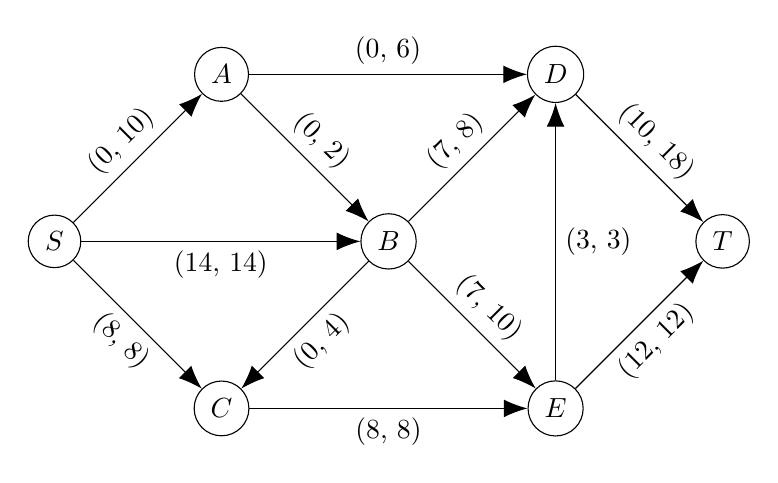
\begin{tikzpicture}[
	node distance = 3 cm,
	vertex/.style = {draw, circle},
	arc/.style = -{Latex[length = 3mm]} % 3mm yerine 3 mm yazarsak dosya dizilmiyor
	% burada "arc/.style = {-{Latex[length = 3mm]}}" demeyip aşağıda her "arc" gördüğümüz yere "-{Latex[length = 3mm]}" yazsak da oluyor
	]
% düğümler
\node [vertex] (S) {$S$};
\node [vertex] (A) [above right of = S] {$A$};
\node [vertex] (C) [below right of = S] {$C$};
\node [vertex] (B) [below right of = A] {$B$};
\node [vertex] (D) [above right of = B] {$D$};
\node [vertex] (E) [below right of = B] {$E$};
\node [vertex] (T) [below right of = D] {$T$};
% arklar
\draw [arc] (S) -- node[midway, above, sloped] {(0, 10)} (A);
\draw [arc] (S) -- node[midway, below] {(14, 14)} (B);
\draw [arc] (S) -- node[midway, below, sloped] {(8, 8)} (C);
\draw [arc] (A) -- node[midway, above, sloped] {(0, 2)} (B);
\draw [arc] (A) -- node[midway, above] {(0, 6)} (D);
\draw [arc] (B) -- node[midway, below, sloped] {(0, 4)} (C);
\draw [arc] (B) -- node[midway, above, sloped] {(7, 8)} (D);
\draw [arc] (B) -- node[midway, above, sloped] {(7, 10)} (E);
\draw [arc] (C) -- node[midway, below] {(8, 8)} (E);
\draw [arc] (D) -- node[midway, above, sloped] {(10, 18)} (T);
\draw [arc] (E) -- node[midway, right] {(3, 3)} (D);
\draw [arc] (E) -- node[midway, below, sloped] {(12, 12)} (T);
\end{tikzpicture}

\bigskip
\hrule
\bigskip

% Düğümler göreceli konumlandırıldığında scale seçeneği çalışmıyor. Onun yerine çizim \resizebox içine alınabilir:
\resizebox{\textwidth}{!}
{ % \resizebox{horizontal length}{vertical length}{material} (burada ünlem işareti "yatay uzunluğa göre boyutlandır" anlamına geliyor)
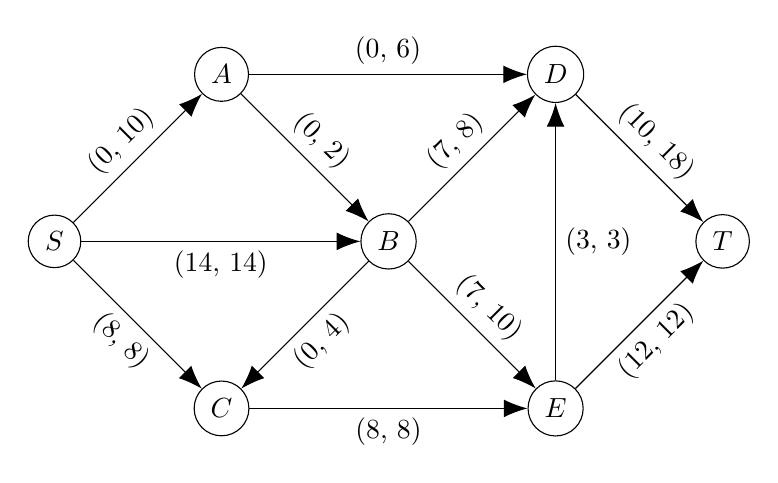
\begin{tikzpicture}[
	node distance = 3 cm,
	vertex/.style = {draw, circle},
	arc/.style = -{Latex[length = 3mm]}
	]
% düğümler
\node [vertex] (S) {$S$};
\node [vertex] (A) [above right of = S] {$A$};
\node [vertex] (C) [below right of = S] {$C$};
\node [vertex] (B) [below right of = A] {$B$};
\node [vertex] (D) [above right of = B] {$D$};
\node [vertex] (E) [below right of = B] {$E$};
\node [vertex] (T) [below right of = D] {$T$};
% arklar
\draw [arc] (S) -- node[midway, above, sloped] {(0, 10)} (A);
\draw [arc] (S) -- node[midway, below] {(14, 14)} (B);
\draw [arc] (S) -- node[midway, below, sloped] {(8, 8)} (C);
\draw [arc] (A) -- node[midway, above, sloped] {(0, 2)} (B);
\draw [arc] (A) -- node[midway, above] {(0, 6)} (D);
\draw [arc] (B) -- node[midway, below, sloped] {(0, 4)} (C);
\draw [arc] (B) -- node[midway, above, sloped] {(7, 8)} (D);
\draw [arc] (B) -- node[midway, above, sloped] {(7, 10)} (E);
\draw [arc] (C) -- node[midway, below] {(8, 8)} (E);
\draw [arc] (D) -- node[midway, above, sloped] {(10, 18)} (T);
\draw [arc] (E) -- node[midway, right] {(3, 3)} (D);
\draw [arc] (E) -- node[midway, below, sloped] {(12, 12)} (T);
% "--" yerine "to" da yazılabiliyor
\end{tikzpicture}
}

\newpage

%%%%%%% SAYFA 3 %%%%%%%

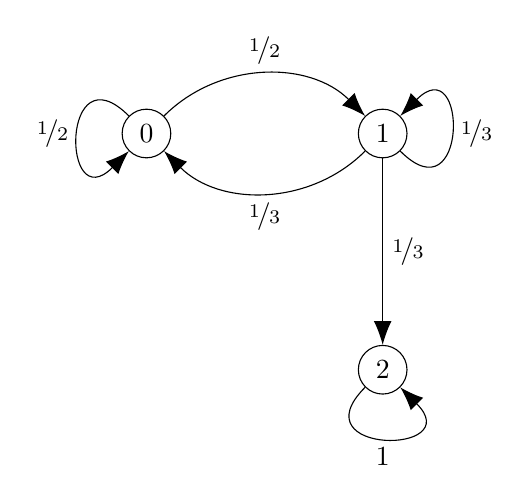
\begin{tikzpicture}[
	node distance = 3 cm,
	state/.style = {draw, circle},
	arc/.style = -{Latex[length = 3mm]}
	]
% düğümler
\node (0) [state] {0};
\node (1) [state, right of = 0] {1};
\node (2) [state, below of = 1] {2};
% arklar
\draw [arc] (0) to [out = 135, in = 225, looseness = 7] node[midway, left] {\nicefrac{1}{2}} (0);
\draw [arc] (0) to [out = 45, in = 135, looseness = 1] node[midway, above] {\nicefrac{1}{2}} (1);
\draw [arc] (1) to [out = 225, in = -45, looseness = 1] node[midway, below] {\nicefrac{1}{3}} (0);
\draw [arc] (1) to [out = -45, in = 45, looseness = 7] node[midway, right] {\nicefrac{1}{3}} (1);
\draw [arc] (1) to node[midway, right] {\nicefrac{1}{3}} (2);
\draw [arc] (2) to [out = 225, in = -45, looseness = 7] node[midway, below] {1} (2);
\end{tikzpicture}

\bigskip
\hrule
\bigskip

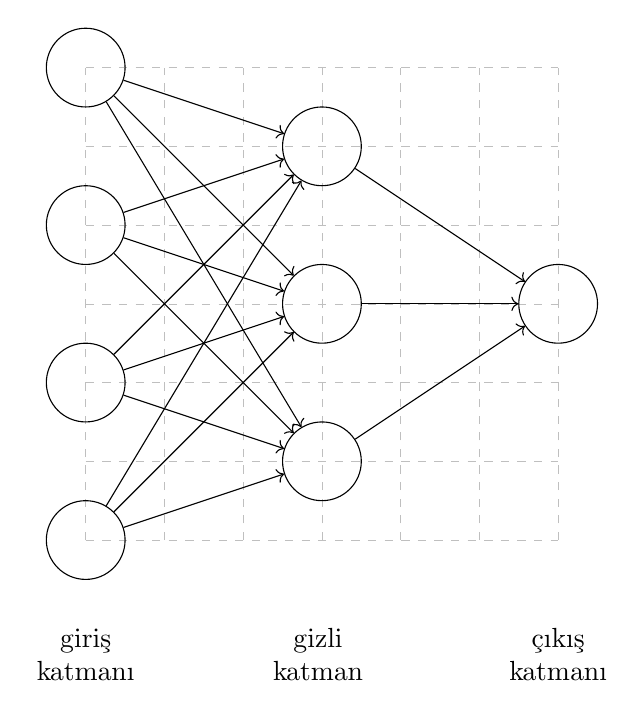
\begin{tikzpicture}[
	node distance = 1 cm and 3 cm, % düşey ve yatay düğüm mesafesi
	neuron/.style = {draw, circle, minimum size = 1 cm}, % minimum size: çizilen çemberlerin asgari çapı
	on grid % katmanlar arası mesafenin birbirine eşit olması için elzem
	]
% yardımcı çizgiler
\draw [help lines, dashed, lightgray] (0, 0) grid (6, -6);
% düğümler (düşey ve yatay düğüm mesafelerinin birbirinden farklı olduğu durumda konum belirtirken "of =" değil "= of" yazmamız gerekiyor)
\node (i1) [neuron] {}; % ilk giriş nöronu (input 1)
\node (h1) [neuron, below right = of i1] {}; % ilk gizli nöron (hidden 1)
\node (i2) [neuron, below left = of h1] {};
\node (h2) [neuron, below right = of i2] {};
\node (i3) [neuron, below left = of h2] {};
\node (h3) [neuron, below right = of i3] {};
\node (i4) [neuron, below left = of h3] {};
\node (o)  [neuron, right = of h2] {}; % çıkış nöronu (output)
% arklar
\draw [->] (i1) -- (h1);
\draw [->] (i1) -- (h2);
\draw [->] (i1) -- (h3);
\draw [->] (i2) -- (h1);
\draw [->] (i2) -- (h2);
\draw [->] (i2) -- (h3);
\draw [->] (i3) -- (h1);
\draw [->] (i3) -- (h2);
\draw [->] (i3) -- (h3);
\draw [->] (i4) -- (h1);
\draw [->] (i4) -- (h2);
\draw [->] (i4) -- (h3);
\draw [->] (h1) -- (o);
\draw [->] (h2) -- (o);
\draw [->] (h3) -- (o);
% katmanlar
\node (n1) [below = 1 cm, align = center] at (i4) {giriş \\ katmanı};
\node (n2) [right = 3 cm, align = center] at (n1.west) {gizli \\ katman};
\node (n3) [right = 3 cm, align = center] at (n2.west) {çıkış \\ katmanı};
\end{tikzpicture}

\end{document}